%%% Local Variables:
%%% mode: latex
%%% TeX-master: "report_main"
%%% End:

\section{Part 2 -- Monovariable control}
%
\subsection{Problem 1}
The following controller form is given in the assignment\cite[p.15]{assignment}:
%
\begin{equation}
  \label{eq:pd_controller}
  \tilde{V_d} = K_{pp}(\tilde{p_c} - \tilde{p}) - K_{pd} \dot{\tilde{p}}
\end {equation}
%
Substituting in the equation for pitch
angle (\cref{eq:pitch EoM}) gives the following.
%
\begin{equation}
  \label{eq:pitch_with_pd}
  \ddot{\tilde{p}} = K_1 K_{pp}(\tilde{p_c} - \tilde{p}) - K_1 K_{pd}
  \dot{\tilde{p}}
\end{equation}
%
To find the transfer
function, $\frac{\tilde{p}(s)}{\tilde{p_c}(s)}$, the Laplace transform
is taken.
%
\begin{align*}
  \ddot{\tilde{p}} + K_1 K_{pd}\dot{\tilde{p}}
  + K_1K_{pp}\tilde{p} &= K_1 K_{pp}\tilde{p_c} \\
  \mathcal{L}\rightarrow&  \\
  s^2\tilde{p}(s) + sK_1K_{pd}\tilde{p}(s)
  + K_1K_{pp}\tilde{p}(s) &= K_1K_{pp}\tilde{p_c}(s)
\end{align*}
%
Which gives the transfer function
%
\begin{equation}
  \label{eq:trans_func}
  \frac{\tilde{p}(s)}{\tilde{p_c}(s)} =
  \frac{K_1K_{pp}}{s^2+K_1K_{pd}s+K_1K_{pp}}
\end{equation}
%
The linearized pitch dynamics can be regarded as a second-order linear
system, which means that by putting \cref{eq:trans_func} in the form
shown in \cref{eq:sol_system}, $K_{pp}$ and $K_{pd}$ can be determine
from $\omega$ and $\zeta$.
%
\begin{equation}
  \label{eq:sol_system}
  h(s) = \frac{\omega^2}{s^2+2\zeta\omega^2s+\omega^2}
\end{equation}
%
This gives the following relations:
%
\begin{align}
  \label{eq:omega}
  \omega &= \sqrt{K_ 1K_ {pp}} \\
  2\zeta\omega^2 &= K_ 1K_ {pd} \nonumber \\
  \label{eq:zeta}
  \zeta = \frac{K_ 1K_ {pd}}{2\omega^2} &= \frac{K_{pd}}{2K_{pp}}
\end{align}
%
For a critically damped system $\zeta = 1$, which gives the following
relationship
%
\begin{equation}
  \label{eq:K_pd}
  K_{pd} = 2K_{pp}
\end{equation}
%
Beginning with a $K_{pp} = 3$, and then from the relation in
\cref{eq:K_pd} a $K_{pd} = 6$, the response of the pitch angle
to the input was slower than desired. Therefore, $K_{pp}$ was
increased to $K_{pp} = 12.5$ and $K_{pd}$ was lowered to underdamp the
system, until it  was sufficiently responsive at $K_{pd} = 0.7K_{pp} =
8.75$. At these values the system responded faster with only minor
oscillations. It was observed that larger values of $K_{pp}$ gave rise
to larger oscillations.
%
\begin{figure}[H]
  \caption{Change in pole position by increasing $K_{pp}$ given a
    constant $K_{pd}$}
  \label{fig:Root_Locus}
  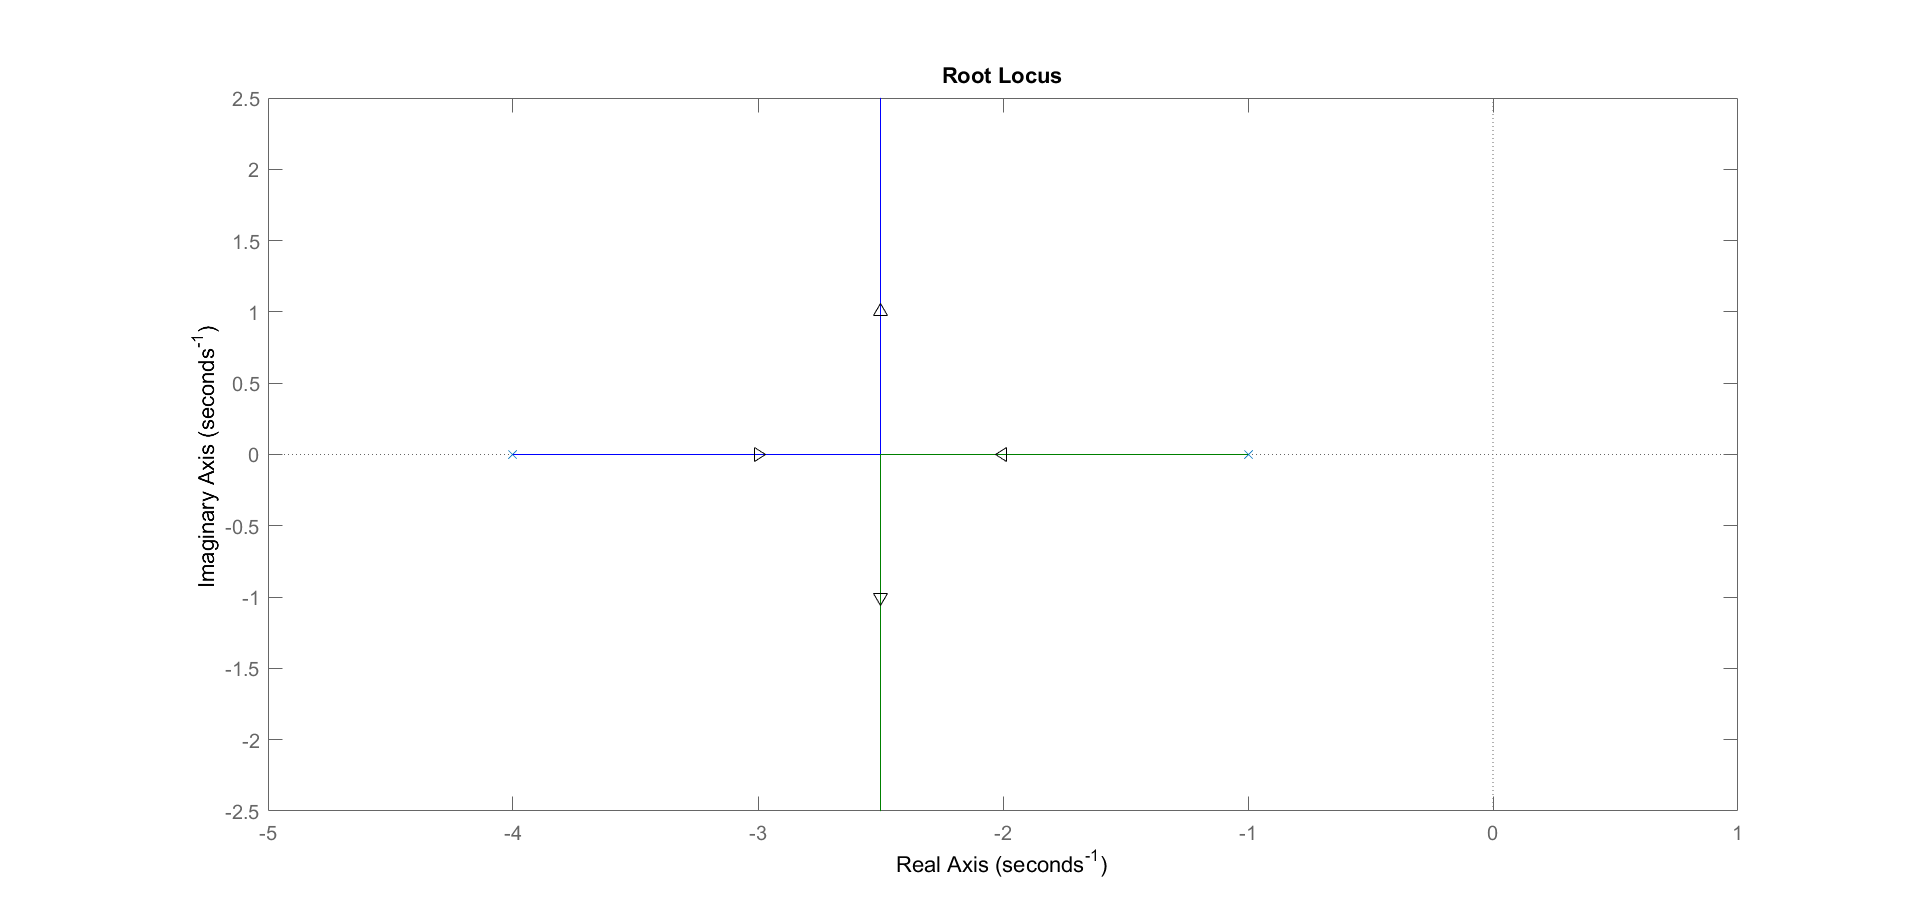
\includegraphics[width=\textwidth]{images/Root_Locus}
\end{figure}
%
At the critically damped point, the poles lie on the same point on
the x-axis. When $K_{pp}$ is decreased in relation to $K_{pd}$ the
system is over-damped the poles move away from each other along the
x-axis. When $K_{pp}$ is increased in relation to $K_{pd}$, the system
is under damped and the poles move away from each other vertically
from the critically damped point.

With the PD controller, it was significantly easier to control the
helicopter than with just feed forward joystick control as no scaling
of the joystick input was needed.

\subsection{Problem 2}
By plugging the P controller for travel
\begin{equation}
\label{travel P controller}
\tilde{p} = K_{rp}(\dot{\tilde{\lambda}}_c - \dot{\tilde{\lambda}})
\end{equation}
into the equation of motion for travel \cref{eq:linearized travel
  EoM}, the transfer function between $\dot{\tilde{\lambda}}$ and
$\dot{\tilde{\lambda}}_c$  can be derived. By substituting the right
side of the controller into the equation of motion for travel the
equation becomes:

\begin{equation}
\label{eq:p controller in travel EoM}
\ddot{\tilde{\lambda}} = K_3(K_{rp}(\dot{\tilde{\lambda}}_c -
\dot{\tilde{\lambda}}))
\end{equation}
After taking the laplace transform and rearranging terms, the transfer
function is as follows:

\begin{equation}
\label{eq:Transfer function between travel and desired travel}
\frac{\dot{\tilde{\lambda}}(s)}{\dot{\tilde{\lambda}}_c(s)} =
\frac{K_3K_{rp}}{s + K_3K_{rp}}
\end{equation}
This controller was quite quick and stable after correctly tuning
$K_{rp}$. The value that was deemed best was $K_{rp}$ = -40. Higher
values, ie. more negative values, of $K_{rp}$ led to large
oscillations, while lower values, or less negative values, of $K_{rp}$
led to a slower response to the joysticks input.  It was necessary
to add a gain to the x value of the joystick to limit the input range
of the controller.

\begin{figure}
  \caption{Simulink implementation of PD controller}
  \centering
  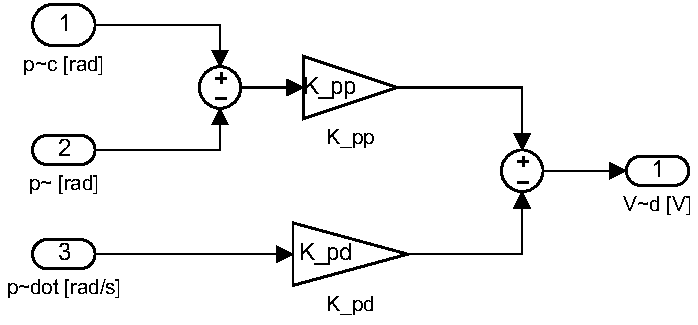
\includegraphics{images/pd_pitch_control.pdf}
  \label{fig:Pitch controller}
\end{figure}

%%% Local Variables:
%%% mode: latex
%%% TeX-master: "report_main"
%%% End:
